\paragraph{Использование информационной избыточности ШПС}
Интересная группа алгоритмов основывается на информационной избыточности ШПС, например \cite{phd_che}. В данной
группе алгоритмов используется механизм появления нескольких точек на основном пике КФ, описанный в \cite{kaplan}. Пример
изображен на рисунке \ref{pic:sec1_peak_tcd}.

\begin{figure}[H]
	\center\scalebox{1}{\includegraphics[width=1\linewidth]{corr_peak_tcd.eps}}
	\caption{Идеальная КФ ШПС с отмеченными точками возможного обнаружения}
	\label{pic:sec1_peak_tcd}
\end{figure}

На рисунке \ref{pic:sec1_peak_tcd} изображен пик КФ с несколькими точками. Две точки находятся выше порога П=0.5.

В работе \cite{phd_che} рассмотрено создание субоптимального обнаружителя на основе информационной избыточности ШПС.
Получена целевая для системы синхронизации в целом и намечены дальнейшие пути развития данного направления.
